% !TEX root = ../main.tex

% = = = = = = = = = = = = = = = = = = = = = = = = = = = = = = = = = = = = = = = = = = = = = = %


%TODO: Expand here

\section{Threat (?) Model}
The attack surface to abuse users' browsers is broad, there are different actors whom can abuse this functionality for their own profit without user consent nor knowledge. There are multiple vectors a malicious actor can inject mining scripts in the website's codebase:

\subsection{Webmaster initiated} 

As discussed before, the website administrator can add the mining script to the webpage without informing users. Website owners may choose to monetize their site with cryptojacking scripts if they have been blacklisted or blocked by standard advertising platforms. In one example, Dutch researcher Sijmen Ruwhof found Coinhive on a large Russian website offering child pornography to users. In this case, revenue estimates, based on the website traffic data available, were roughly \$10,000 a month after converting the value of XMR mined to USD~\cite{coinhiveonchildporn}

\subsection{Ad network} 

Similar to the claimed Showtime case~\cite{showtimehive}, the advertisement publisher can inject miner script to any website they have ad space in instead of showing legitimate ads (more on this in User Impact section).

\subsection{Breached website} 
An attacker can hack a service provider's codebase and inject their mining code to the one or many websites at once, simply turning access to money. A recent example of this type of attack, discovered on Thanksgiving Day by security researcher Troy Mursch, occurred to LiveHelpNow's SDK that resulted in unsolicited mining when accessing their chat system through all website using the char support service~\cite{chatsupporthack}.

On October 13, Coinhive was found on the political fact-checking website Politifact\footnote{PolitiFact: Fact-checking US politics \url{https://politifact.com/}}. A compromised JavaScript library was found to be injecting the cryptojacking scripts. The malicious code remained on the site for at least four hours before it was removed~\cite{politifactcoinhive}. In a statement provided to The Wall Street Journal, PolitiFact Executive Director Aaron Sharockman stated ``Hackers were able to install their script on the fact-checking website after discovering a misconfigured cloud-computing server.`` ~\cite{politifactcoinhivewsj}.

\subsection{Man-in-the-middle attack} 

Any internet service provider or free public wireless connection can inject the script to all the plain text traffic that goes through their routers. Advertisement code injection has been seen in practice ~\cite{vergeadinjection}. Also there have been reports of similar injections of browser mining scripts at certain Starbucks free Wi-Fi hotspots\footnote{\url{https://twitter.com/imnoah/status/936948776119537665}}.

In two separate incidents, Coinhive was injected into the websites of Globovision\footnote{Globovision is a 24-hour television news network in Venezuela and Latin America.\url{http://globovision.com/}} and Movistar\footnote{Movistar is a major telecommunications brand owned by Telefonica, operating in Spain and in many Hispanic American countries \url{https://www.movistar.com/}} using Google Tag Manager\footnote{Google Tag Manager is a tag management system created by Google to manage JavaScript and HTML tags used for tracking and analytics on websites}. Movistar stated that Coinhive was not put on their website by a hacker, but instead was due to \textit{``internal error``} while they were conducting ``production tests``. No statement was provided by Globovision on why the cryptojacking scripts appeared on their site on November 15, 2017~\cite{googletagcoinhive}.

\subsection{Other Browser related vectors} %TODO: maybe a better title? or even just in discussion?
Cryptojacking was not limited to websites in 2017 as we saw Chrome extensions also being affected. One such extension, Archive Poster, remained on the Chrome Web Store for days while silently cryptojacking an unknown portion of their 100,000+ users. Despite multiple user reports, Google`s security team did not remove the extension until multiple news media outlets covered the issue~\cite{chromeextentioncoinhive}. 

One possible solution is to enforce user consent on service provider level. One example for this is that Coinhive started Authedmine to enforce user consent before running the miners, Although Clickjacking~\cite{rydstedt2010busting} and other methods of obfuscation has been used to bypass this enforcement model and run the miner code without the proper authorization.


% = = = = = = = = = = = = = = = = = = = = = = = = = = = = = = = = = = = = = = = = = = = = = = %


\section{Measurements}

\subsection{Prevalence}

In order to find out how browser mining is changing internet use, the approach taken was to find measurements of the impact it causes. One approach was to see what the search interest over time for such services is. 

\begin{figure}[t]
\centering
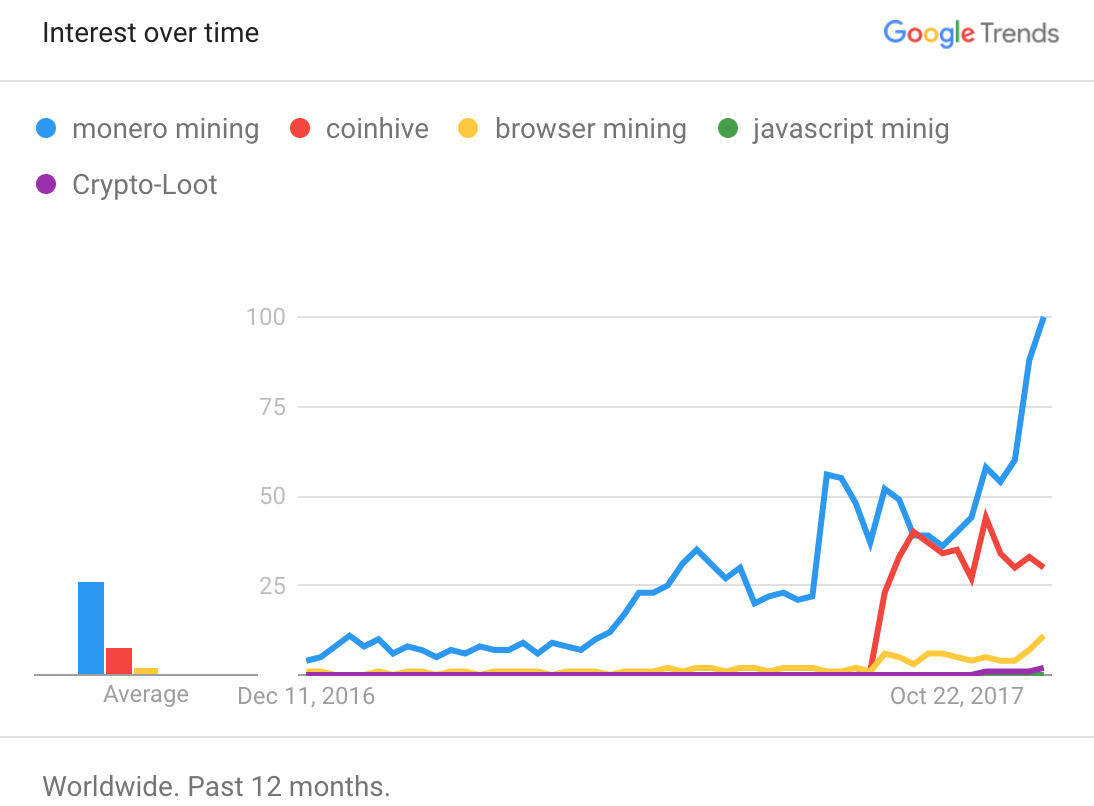
\includegraphics[width=\linewidth]{figures/usage_over_time2.png}
\caption{Google Trend - Search interest over last 12 months}
\end{figure}

It seems that there has been more interest in Coinhive than the broader, related search term ``Browser mining''. Comparing to other services offering Monero browser mining API, Coinhive had the advantage of being the first to offer the service, hence more interest at the time of writing. There has not been enough data and evidence of usage for other services to analyze, thus the focus of this paper is on the impact of Coinhive scripts on the internet. 

The next step was to see how many websites are deploying Coinhive scripts by using internet scanners such as Zmap\footnote{\url{https://zmap.io}}. It was of more interest to see what the trend of this usage was, and for this purpose historical data was required. 

\begin{lstlisting}[caption={BigQuery SQL query to find websites using coinhive miner script using censys.io datasets},label={lst:bigquery},language=sql,linewidth=\linewidth]

SELECT domain, tags, p80.http_www.get.headers.content_language, p80.http_www.get.headers.server, p80.http.get.headers.x_powered_by, p80.http.get.title, p80.http_www.get.body as wwwbody, p80.http.get.body as plainbody 
FROM censys-io.domain_public.20171123
WHERE STRPOS(p80.http.get.body, coinhive.min.js) > 0 or STRPOS(p80.http_www.get.body, coinhive.min.js) >0)

\end{lstlisting}

Using censys.io BigQuery dataset ~\cite{censys15}, it is feasible to query for such trends. The method used to gather these data is simply looking for the `coinhive.min.js` script within the body of the website page. These findings are corroborated by another search engine, PublicWWW, which indexes the source code of publicly available websites. Using PublicWWW's dataset, over 30,000 websites were found to have the `coinhive.min.js` library~\cite{badpacketspublicwww}.
 
However, cryptojacking services are evolving to use obfuscated JavaScript and randomized URLs to evade detection\footnote{\url{https://twitter.com/bad_packets/status/940333744035999744}}. An example of these methods can be found in the cryptojacking service provider called Minr. In this case, the script is automatically obfuscated for users implementing the code. In addition, the domain names used by Minr frequently change to circumvent blocklists and anti-malware software.

\begin{figure}[t]
\centering
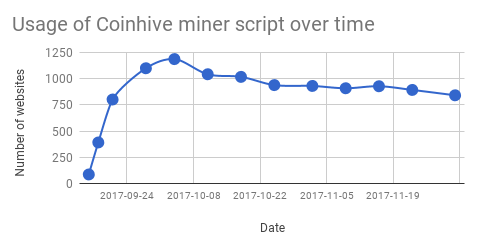
\includegraphics[width=\linewidth]{figures/usage_of_coinhive_over_time.png}
\caption{Usage of CoinHive Miner scripts in top 1 million websites over time}
\end{figure}


As seen in the chart above, the adoption of this script was substantial in the first days of its release. However, progress slowed down as ad-blockers and organizations started to block Coinhive's website. The initial purpose of this service, as claimed by Coinhive, was to replace ads and cover server costs for webmasters. As the service did not require that website's received user consent before beginning to mine, it started to be used maliciously in user`s browsers. This type of usage resulted in Coinhive being included in the top-10 most wanted malware list after some famous ransomware ~\cite{checkpoint}. 

\begin{figure}[t]
\centering
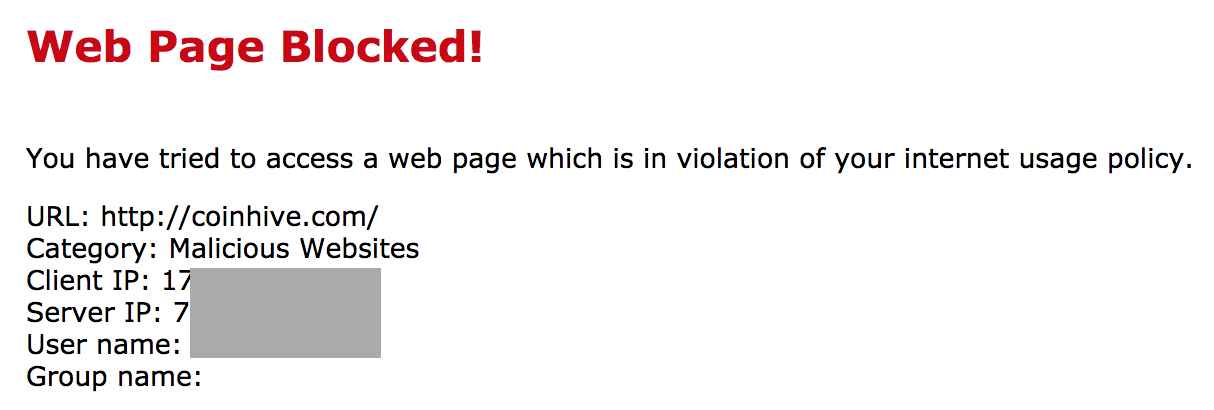
\includegraphics[width=\linewidth]{figures/coinhive_blocked.png}
\caption{Our university has blocked coinhive.com website}
\end{figure}


This helped Coinhive copycats gain some market attention as they came online late in 2017. Increased competition pushed Coinhive developers to think of other methods that would be more focused on user consent and bypassing blockage for running such scripts.

\begin{figure}[t]
\centering
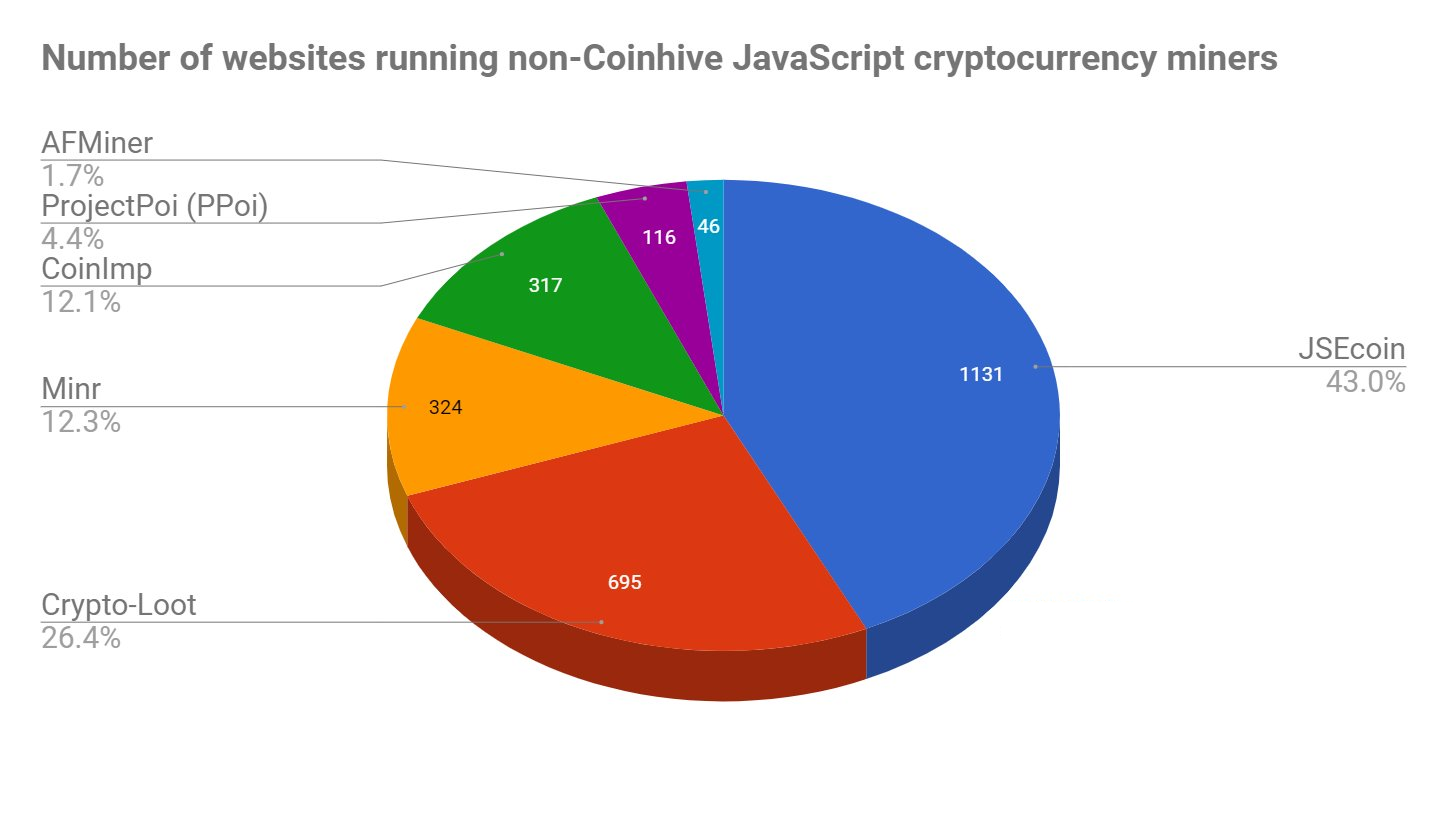
\includegraphics[width=\linewidth]{figures/non-coinhive-miners.png}
	\caption{Copycats of coinhive}
\end{figure}



\subsection{Clientside Impact}

\begin{figure}[t]
\centering
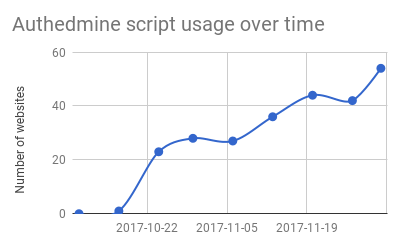
\includegraphics[width=\linewidth]{figures/usage_of_authedmine_over_time.png}
	\caption{Usage of AuthedMine Miner scripts in top 1million websites over time}
\end{figure}

Coinhive introduced another domain and service called ``Authedmine'' , which requires user`s consent to start mining in the browser. This service did not get the same attention as the original service, but it did inspire discussions regarding the ethics of such services, which is covered in Discussion section of this paper. (Clickjacking) 

Most of these scripts discovered were configured to use around 25\% of user`s CPU, which can be justified as it will be under the threshold of attracting the user`s attention, and it could be argued as fair-usage of their hardware. During the first few days, however, there were some reports of 100\% CPU usage when visiting websites containing these scripts~\cite{piratesbayblog}, which can be characterized as malicious. By default, the Coinhive JavaScript library will use all available CPU resources available. The user implementing the script must include a throttle value to reduce the client-side CPU usage during mining operations.

\begin{figure}[t]
\centering
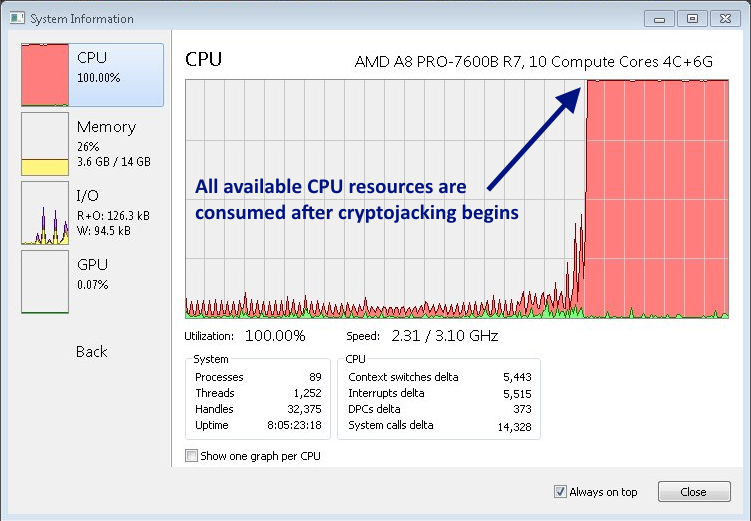
\includegraphics[width=\linewidth]{figures/windows_cpu_usage.png}
	\caption{Comparison of CPU usage of browser without and with browser mining enabled}
\end{figure}

\subsection{Profitability}
\label{profitabilitexperiment}

Coinhive developers estimate a monthly revenue of about 0.3 XMR (~\$101) for a website with 10-20 active miners, which would be users with longer duration of visit on the website~\cite{coinhive}.

Through correspondence with one of the biggest coinhive campaigns operator, which was a domain parking service and was running coinhive script on over 11,000 parked websites, conducted over period of three months, we were able to gather some data to estimate profitability for websites with high traffic but short visits \footnote{Collaborated with Faraz Fallahi \url{https://github.com/fffaraz}}. Over 97,000 users visited these websites for an average of 24 seconds per session.


%TODO: Separate these charts

\begin{figure}[t]
\centering
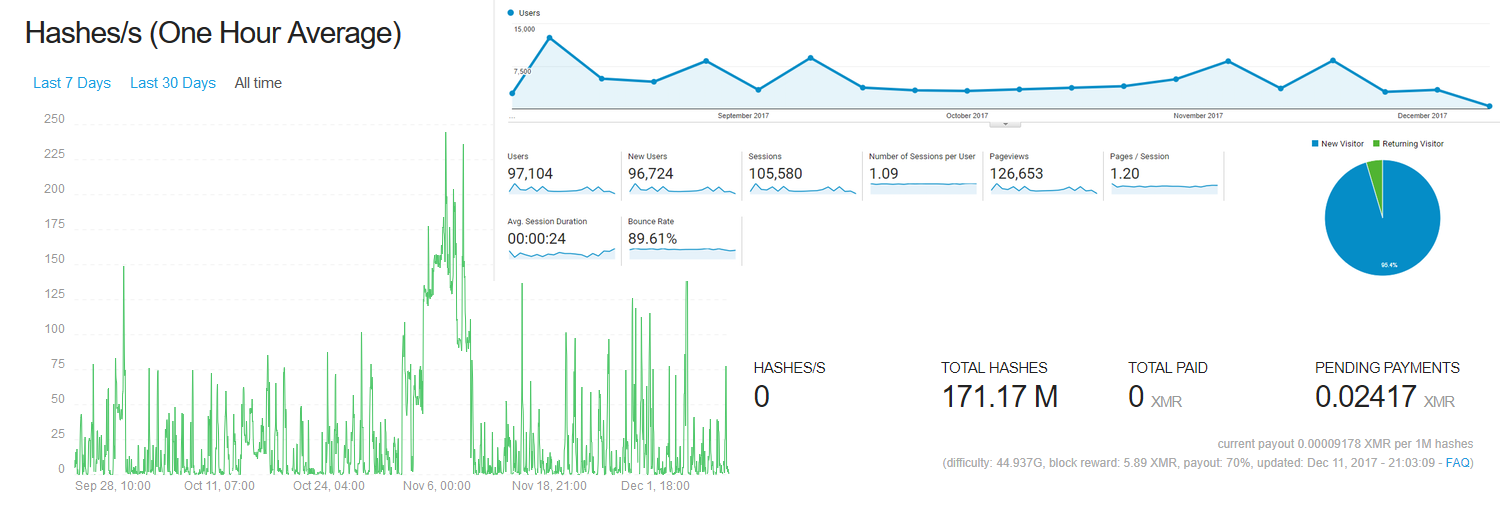
\includegraphics[width=\linewidth]{figures/coinhive_experiment_11k.png}
\caption{Results from Coinhive and Google Analytics dashboards}
\end{figure}

This experiment showed that even though the number of users visiting was significant, the profit from those visits was below expectations. For the period examined, the revenue was 0.02417 Monero, which at the time of writing is equivalent to 7.69 USD.


% = = = = = = = = = = = = = = = = = = = = = = = = = = = = = = = = = = = = = = = = = = = = = = %


\section{Ethical Considerations}

The opinion of the authors of this paper maintain that users should be given the option to enable the miner code in their browser only with some benefit to their experience on the website.  An example of a benefit could be the removal of advertisements. Recent polls support this notion, such as the one conducted by Bleeping Computer, which found that ``many users said they are OK with websites mining Monero in the background if they don`t see ads anymore''~\cite{bleepingcomputerminers}. Another example would be granting access to premium features of the website such as journal articles behind a paywall, or streaming in high-definition. The website could also allow the user to participate in mining rewards by allocating a large portion of their CPU resources to the activity of mining, which would benefit both parties. By notifying the user of the potentials of such activity, and allowing them to make a choice to participate, the website maintains trust in their relationship with the user while also benefiting from a new source of revenue. By foregoing disclaiming this new activity, which can have harmful effects, the website will gain a new revenue stream for a short time only while sacrificing their reputation in the long term. Coinhive`s recent response to the market`s negative reaction by releasing AuthedMine, which enforces user consent before enabling any mining JavaScript code, justifies this rationale. However, before consented browser mining could develop into a sustainable model, its security implications and user impact should be addressed.
Browser developers are starting to talk about throttling or blocking such scripts\footnote{Please consider intervention for high cpu usage js \url{https://bugs.chromium.org/p/chromium/issues/detail?id=766068}}, however this discussion need further considerations as throttling should happen based on some variables, in which might affect legitimate applications as well. Also if they switch to user notification for high CPU usage per website, the notification itself might not be affective as desired~\cite{SHB11}\cite{SEAAC09}.

Coinhive as a big player in the recent rise of in-browser mining, introduced its functionality as a replacement for online advertisement, a new way to monetize website`s traffic. However this will result in a paradigm shift in website monetization. As an example in both auction-based and keyword-based online advertisement, the advertiser pays the ad publisher to distribute the ads and the ad publisher pays a portion of the revenues to the website owner whom the ad was shown on her website~\cite{king2007internet}. However in in-browser mining as a replacement monetization strategy, user is technically paying for the visit on their hydro (electricity) bill, in which the consent of the user becomes an ethical issue. As the concept of traffic revenue begins to change, the values associated with the old concept will have to be reexamined. Moor, in "What is Computer Ethics?" ~\cite{moor1985computer} introduces the concept of \textit{Invisible Factor}, for invisible computer operations in society. Based on his definitions cryptojacking falls under \textit{Invisible abuse}\footnote{The intentional use of the invisible operations of a computer to engage in unethical conduct}. Here the cryptojacker is earning money from unaware users that are being charged on their hydro bill. 

Most browser mining code is ran without the consent, nor knowledge, of the users involved. As previously mentioned, the websites that have been found running JavaScript code for the purpose of mining usually employed Coinhive`s API. One such website, for example, ThePirateBay.org~\cite{bbcmintcrypto}, which ran the JavaScript code when users searched for torrent files. Perhaps unsurprisingly, there was no notice in their Privacy Policy nor visible warning on any part of the website that informed their users of this activity. This resulted in a backlash against the website, which responded with the following statement, ``Do you want ads or do you want to give away a few of your CPU cycles every time you visit the site?'' ~\cite{piratesbayblog}. While they admitted to their testing of browser mining, their notice came after the fact and resulted in the removal of the JavaScript code altogether due to upset users. This is in contrast to the banners users are presented with upon the first visit to a website that warns them of the website`s policy on cookies, which is enforced today through EU laws~\cite{eucookie}. It is now widely known that these cookies can be used to track users across the internet, so cookie banners can act as a reminder and allow the user to make better informed decisions regarding their browsing habits. Without any type of disclaimer for users, websites have been commandeering their users` CPU resources for their business and personal gain. This results in higher energy bills for the user, along with accelerated device degradation, slower system performance, and poor web experience\footnote{The Performance Impact of Cryptocurrency Mining on the Web \url{https://discuss.httparchive.org/t/the-performance-impact-of-cryptocurrency-mining-on-the-web/1126}}~\cite{gaurdianelectricity}.

A second example of a popular website deploying Coinhive�s API is Showtime.com, which is a popular cable channel that also streams their TV shows online. Showtime has declined to comment on how or why Coinhive was implemented on their website. Speculation has been raised that it was injected via an third-party analytics tool, New Relic, due to Coinhive being found inside the New Relic code block within website's source code. However a New Relic representative denied these claims in a statement to The Register, "It appears they [Coinhive scripts] were added to the website by its [Showtime's] developers." ~\cite{registershowtime}. 

It was then hardly surprising when UFC.com was accused of using this very same code on the night of streaming one of their most popular events~\cite{registerufcmonero}. In a statement released by the UFC, they denied the presence of the code stating, ``[they] did not find any reference to the mentioned Coinhive JavaScript [code]``\footnote{\url{https://twitter.com/bad_packets/status/928044219222048769}}.
 
The recent trend of streaming websites deploying Coinhive's API could be due to the high costs of providing streaming services. While ads can be used to offset some of those costs, it would be of interest to some to at least experiment with the idea of recruiting their users to mine Monero for profit. This same regard is true for hackers looking to maximize their cryptojacking profits. The longer a user is engaged on a website, such as video streaming service, the more income can be earned through browser mining.

Given the recent interest some websites have shown in regard to browser mining, there is also potential for this new form of revenue generation to compete with advertisements. As seen in section~\ref{profitabilitexperiment}, an immediate impact could be to reduce how many ads a user sees on a given website. Moving forward websites with long user sessions such as streaming services could one day even replace ads. This is because the malware that is associated with advertisements is still a growing concern, and the public`s dislike of advertisements will likely persist and not wane. Also, as cryptocurrencies continue to grow in market capitalization and use cases, their inevitable mainstream use will push the profitability of mining egalitarian proof-of-work cryptocurrencies, such as Monero, well into the future. There are many ongoing discussions on the potential of browser mining one day replacing online advertisement\footnote{Carl Whalley - Could cryptocurrency kill online advertising \url{https://www.linkedin.com/pulse/could-cryptocurrency-kill-online-advertising-carl-whalley}}.
%The lack of regulation in cryptocurrency space allows for a grey market to grow. This is felt more when it affects non-tech-savvy users. 


% = = = = = = = = = = = = = = = = = = = = = = = = = = = = = = = = = = = = = = = = = = = = = = %

\section{Mitigations}

Similar to regulations for cookies and user tracking there is a need to regulate browser mining, primarily to notify users of the existence of these scripts on the webpages they visit. Also, there is a need to standardize this model, so to answer some of these questions: If every website uses a browser miner and users have many tabs open, how are CPU resources shared between them? How will the behaviour of these scripts change based on the device they are running on? If device is on power saving mode, how will that affect the execution of these scripts?

In addition to regulation and standardizing, better security design is required to narrow down the attack surface, such as using SSL/TLS and tokenizing the requests to make sure websites get user`s consent before running these scripts. DNS TXT records could also be implemented to verify domain name ownership before browser mining scripts would be authorized to run on the website.

Surveys with larger sample size and diversity is required to gauge users acceptance. These surveys should answer how much CPU power users are willing to volunteer, and if battery impact would change their affinity for participation.

Browser mining has been shown to not be as efficient as native mining applications today. Therefore, optimizations on how browsers pass system calls to the operating system can be made, or there can even be browsers designed specifically to support efficient browser mining. However, browsers such as Opera, have taken a stance against cryptojacking scripts and blocked them via "NoCoin" blacklist ~\cite{operanocoin}. The effectiveness of using a blacklist to block such activities is still not clear. %maybe a bit more on this? meaning that as seen so far, cryptojackers can just use new domains/ips to bypass these blacklists

This new model of monetizing websites can be a paradigm shift in how advertisement giants monopolize internet traffic. This could lead to re-democratizing the online advertisement ecosystem to make it fairer for smaller players.

% = = = = = = = = = = = = = = = = = = = = = = = = = = = = = = = = = = = = = = = = = = = = = = %

\section{Concluding Remarks}



















